\documentclass{article}
\usepackage{geometry}
\geometry{a4paper, margin=1in}
\usepackage{hyperref}
\usepackage{fancyhdr}
\pagestyle{fancy}
\usepackage{enumitem}
\usepackage{graphicx}
\fancyhead[L]{STAT 3611 Assignment (Lab 1)}
\fancyhead[R]{Jan 20 at 11:59pm}
\setlist[itemize]{topsep=2pt, itemsep=1pt, left=10pt}
\setlist[enumerate]{topsep=2pt, itemsep=1pt, left=10pt}

\begin{document}

\section*{Topic Overview}
In this lab, you will install R and familiarize yourself with the interface and basic syntax in R by using the \texttt{swirl()} library tutorials.

\section*{Submission Instructions}
For this lab, you will submit \textbf{2 files}:
\begin{enumerate}
    \item Your “code” file must have a \texttt{.pdf} extension and be named \texttt{Lab1\_Console\_LastNameFirstName.pdf}.
    \item Your notes file must have a \texttt{.pdf} extension and be named \texttt{Lab1\_Notes\_LastNameFirstName.pdf}.
\end{enumerate}

\section*{Lab Instructions}
\subsection*{Installing and Accessing R}
Because R is free and open source, it is highly recommended that you install R and R Studio on your own computer. This program is also available on the lab computers in \texttt{Parker Hall 126} and on the College of Engineering virtual lab.

Links and instructions to download R and R-Studio can be found in \href{https://swirlstats.com/students.html}{Step 1 and Step 2 of the instructions here}.

\subsection*{Set Your Working Directory in R Studio}
It is highly recommended that you make a folder on your computer to store all of your files for this class and then choose that folder as your working directory.

\begin{verbatim}
session > set working directory > choose directory
\end{verbatim}
\begin{center}
    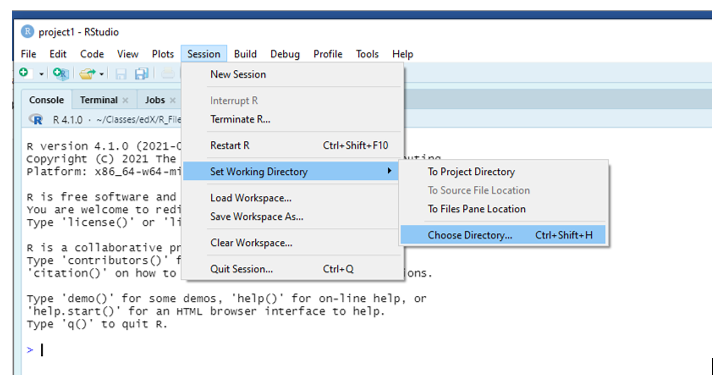
\includegraphics[width=0.5\textwidth]{3611_p1.png}
\end{center}

You will see your new working directory in the R console after this step, as shown below:

\begin{center}
    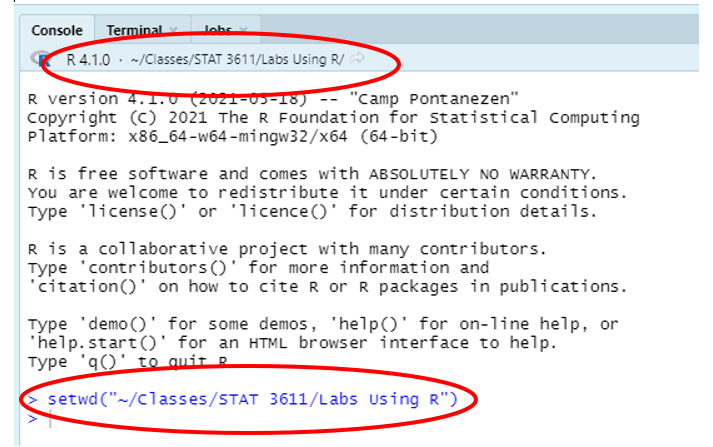
\includegraphics[width=0.5\textwidth]{3611_p2.png}
\end{center}

\subsection*{Completing the \texttt{swirl()} Tutorial}
The \texttt{swirl()} library will walk you through the basics of R syntax and data types. Some things will feel very familiar because they are similar to Matlab; others will be new ways of working with data.

\textbf{Instructions:}
\begin{enumerate} 
    \item  As you work through the swirl tutorial, create a 1 page (1 sided) note sheet for yourself that you can use as a reference sheet as you complete the rest of the labs this semester.  You may hand-write or type your note sheet.  This note sheet will be submitted as part of your lab report.  

    \item Install \texttt{swirl} following Step 3 of the instructions linked above and load the library:
    \begin{verbatim}
    install.packages("swirl")
    library(swirl)
    \end{verbatim}
    \item Install the course \texttt{R Programming E}:
    \begin{verbatim}
    install_course("R Programming E")
    \end{verbatim}
    More detailed instructions can be found \href{https://github.com/swirldev/swirl_courses#swirl-courses}{here}.
    \item Launch \texttt{swirl}:
    \begin{verbatim}
    swirl()
    \end{verbatim}
\end{enumerate}
Note: Your console will look something like this once you have swirl and the R Programming E course installed.
\begin{center}
    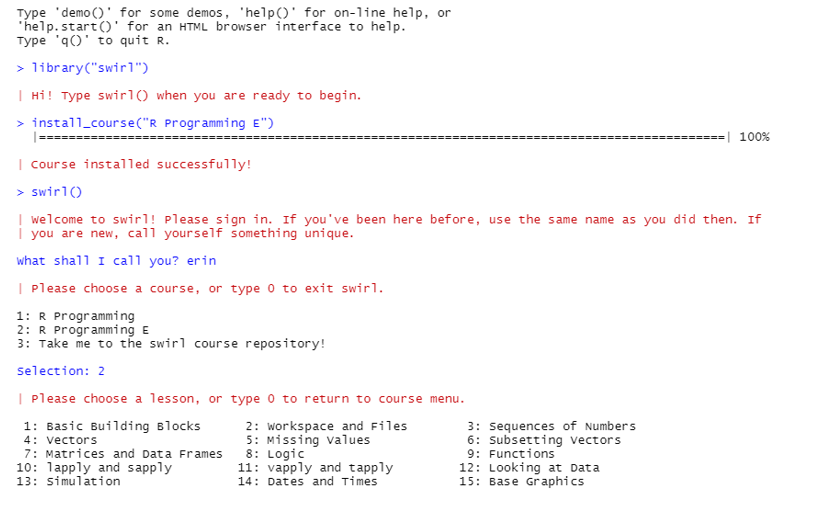
\includegraphics[width=0.5\textwidth]{3611_p3.png}
\end{center}

\textbf{Required Tutorials:}
\begin{itemize}
    \item Tutorial 1: Basic Building Blocks (about 15 minutes)
    \item Tutorial 3: Sequences of Numbers (about 5 minutes)
    \item Tutorial 4: Vectors (about 10 minutes)
    \item Tutorial 5: Missing Values (about 5 minutes)
    \item Tutorial 6: Subsetting Vectors (about 10 minutes)
    \item Tutorial 7: Matrices and Data Frames (about 10 minutes)
    \item Tutorial 12: Looking at Data (about 5 minutes)
\end{itemize}
Complete the avobe tutorials, and note that this entire lab will be done in the R Console. You can also use the Rstudio.  Future labs will be written as scripts that can be saved and run again.

Once you get to the end of each tutorial, you will be asked if you want to inform anyone about the completion, select no.  Example below
\begin{center}
    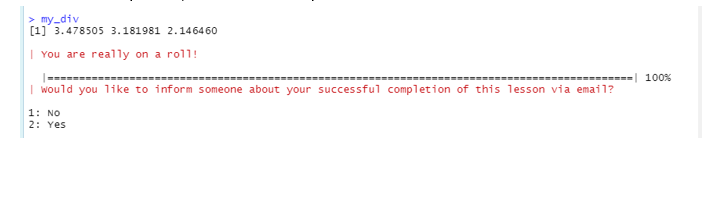
\includegraphics[width=0.8\textwidth]{3611_p4.png}
\end{center}


To create your Console documet, you will need to copy the code from the R Console into a word processing document.  You do not have to complete all of the required swirl tutorials in one sitting, but you must compile the console text from all of the required tutorials into one document.  Once you have completed them all and put all of the console lines into one word processing document, export that document as a pdf for submission. 

The easiest way to copy all of the lines from the console is to right click in the console and choose “select all” from the menu options.  Then right click again and select “copy”.
\begin{center}
    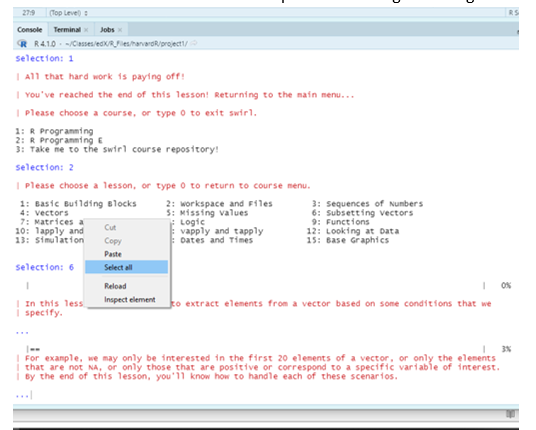
\includegraphics[width=0.5\textwidth]{3611_p5.png}
\end{center}

Then you can paste into your word processing software by right clicking and select the paste text only option.  There will be a lot of white space in the resulting document, this is fine because we won’t be printing a paper copy of the reports for this lab so you don’t need to do any additional formatting work for the report. 
\begin{center}
    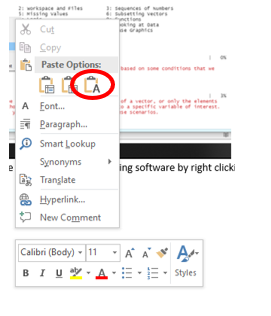
\includegraphics[width=0.4\textwidth]{3611_p6.png}
\end{center}

\newpage
\textbf{Notes:}
\begin{itemize}
    \item Create a one-page (1-sided) note sheet as a reference for the semester. You may hand-write or type this note sheet.
    \item Copy all console lines from the tutorials into one document and save it as a \texttt{.pdf} for submission.
    \item You can temporarily leave a lesson by typing \texttt{play()} and return by typing \texttt{nxt()}.
\end{itemize}
\section*{Grading}
\begin{itemize}
    \item \textbf{50 points:} Completion of the \texttt{swirl} tutorials and submission of the R console as a \texttt{.pdf}.
    \item \textbf{50 points:} R notation and key notes sheet drafted and submitted as a \texttt{.pdf}.
\end{itemize}

\end{document}
